% !TeX root = ../../main.tex
\newpage
\section{Zaproponowana architektura sieci}
\label{sec:zaproponowana_architektura}

Ze względu na to, iż niewystarczająco dokładna detekcja obszaru kortu może niekorzystnie wpływać na wynik meczy oraz ze względu na fakt, iż oprogramowanie może być uruchamiane na przenośnych komputerach, w ramach niniejszej pracy implementacja \textit{Mask R-CNN} została zmodyfikowana w następujących krokach:

\begin{itemize}
	\item architektura sieci została zmodyfikowana w celu osiągnięcia wyższej dokładności maski, poprzez dodanie konfigurowalnej hiperparametrem $deconv\_layers$ liczby warstw dekonwolucyjnych.;
	\item wprowadzony hiperparametr sieci $deconv\_layers$ został dobrany w taki sposób, aby osiągnąć jak najwyższą dokładność maski jednocześnie nie przekraczając pamięci GPU używanej przez autora karty graficznej.
\end{itemize}

Implementacja \textit{Mask R-CNN} opisana w Rozdziale \numberref{sec:maskrcnn} okazała się niewystarczająca na potrzeby systemu automatycznego sędziowania meczór badmintona ze względu na zbyt niską dokładność detektowanej maski.
Maska generowana przez sieć neuronową w implementacji \cite{matterport-mask-rcnn} o rozdzielczości 28x28 pikseli, która na koniec zostaje przeskalowana do odpowiednio większego rozmiaru, okazuje się niewystarczająco dokładna w przypadku obrazów ze zbiorów danych \textit{low} i \textit{high}.
Problem zilustrowany został na Rysunku \numberref{fig:falbanki_original}. 

\begin{figure}[!htb]
  \minipage{0.45\textwidth}
    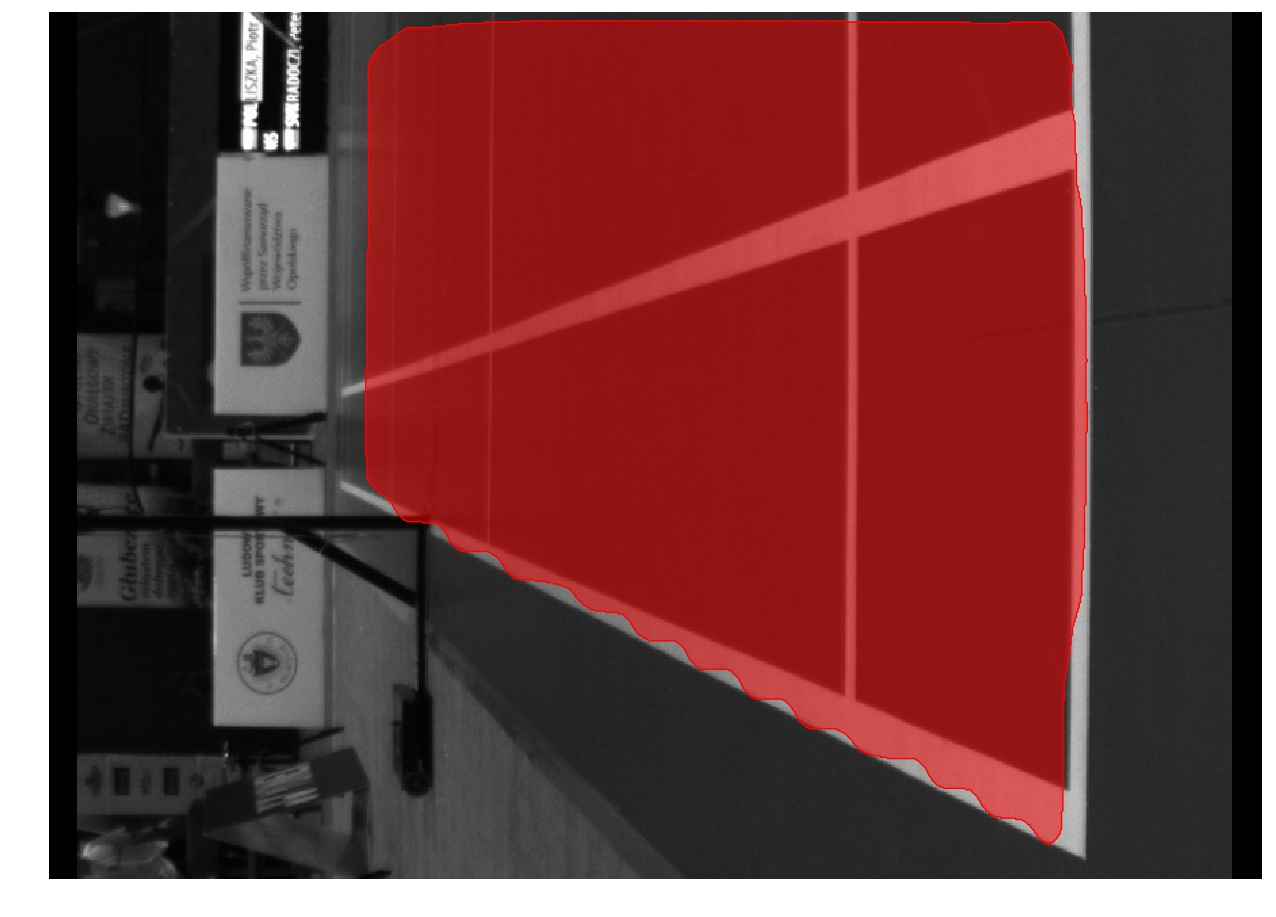
\includegraphics[width=\linewidth]{./original_result_frame_45.jpg}
    \caption{Wynik detekcji maski na obrazie ze zbioru \textit{low} przy użyciu oryginalnej sieci \textit{Mask R-CNN}}
    \label{fig:falbanki_original}
  \endminipage\hfill
  \minipage{0.45\textwidth}
    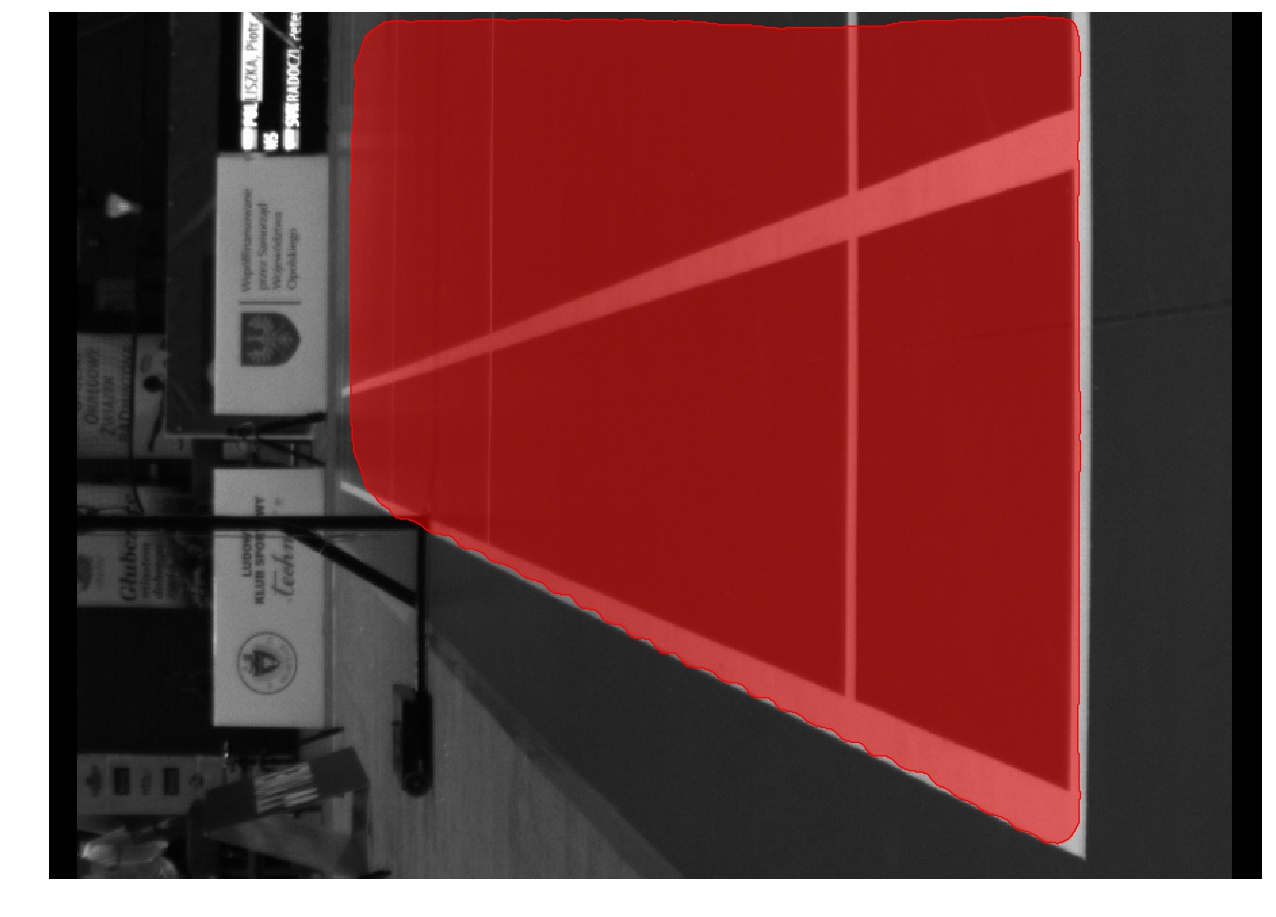
\includegraphics[width=\linewidth]{./56_result_frame_45.jpg}
    \caption{Wynik detekcji maski na obrazie ze zbioru \textit{low} przy użyciu zmodyfikowanej sieci \textit{Mask R-CNN}}
    \label{fig:falbanki_56}
  \endminipage\hfill
\end{figure}

Modyfikacja implementacji \textit{Mask R-CNN} polega na dodaniu hiperparametru $deconv\_layers$, który pozwala na konfigurowanie liczby warstw dekonwolucyjnych w podsieci modelu dotyczącej detekcji maski.
Pseudokod \numberref{alg:mask-r-cnn-modified} przedstawia w jaki sposób powstaje ta podsieć. Co istotne, w przypadku przyjęcia wartości hiperparametru $deconv\_layers = 1$, działanie zmodyfikowanego kodu jest tożsame z działaniem oryginalnej implementacji, opisanej w pseudokodzie \numberref{alg:mask-r-cnn}.

Eksperymenty z dobieraniem wyższej wartości $deconv\_layers$ pokazały, iż wartości $deconv\_layers = 3$ i większe powodują przekroczenie dostępnej pamięci GPU na używanej karcie graficznej\footnote{Używana karta graficzna to \textit{GeForce GTX 1080} z 8GB dostępnej pamięci, użyczona przez firmę \blue{}}.
W związku z powyższym za wartość hiperparametru zmodyfikowanej sieci we wszystkich eksperymentach opisanych w Rozdziale \numberref{sec:eksperymenty_wyniki} przyjęto $deconv\_layers = 2$. Z takim doborem hiperparametru rozdzielczość maski generowanej przez sieć wynosi 56x56 pikseli, co daje dokładniejsze wyniki, zilustrowane na Rysunku \numberref{fig:falbanki_56}.

\vspace{0.5cm}

\begin{algorithm}
  \subimport{mask_r-cnn/}{commoninput}
  \hspace*{\algorithmicindent} \verb|deconv_layers| - \deconvlayersdescription \\
  \subimport{mask_r-cnn/}{commonoutput}
  \begin{algorithmic}[1]
    \subimport{mask_r-cnn/}{firststepsofmask}
    \For {$\mathit{i} = 1$ to deconv\_layers }
      \State $\mathit{L} \gets [...L,\verb| deconvolution 2x2 with strides 2|]$
    \EndFor
    \subimport{mask_r-cnn/}{laststepsofmask}
	\end{algorithmic}
	\caption{Tworzenie podsieci maski w większej rozdzielczości}
	\label{alg:mask-r-cnn-modified}
\end{algorithm}
